\section{Dashboard}
Dashboardet udvikles for at have et sted at samle alle widgets for en gruppe. Det indebærer at linke til de views, hvori man kan redigere og slette de forskellige widgets, herudover skal dashboardet kunne varetage opgaven fra US  tilføj widget, som giver en bruger mulighed for at tilføje/lave en widget til gruppen. US'en "tilføj widget" kan findes på tabel \ref{tab:US_rep}. \\

\begin{figure}[H]
    \centering
    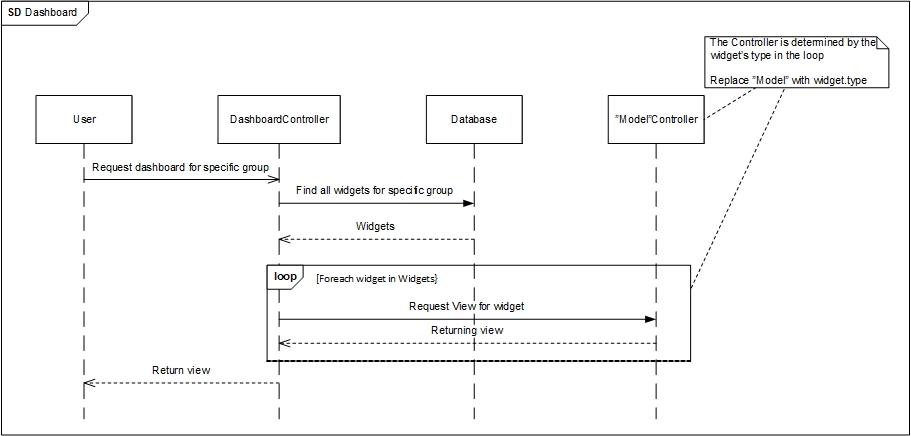
\includegraphics[width=1\textwidth]{09_Arkitektur/Dashboard/Sekvens.jpg}
    \caption{Denne figur viser et sekvensdiagram over udskrivelsen af widgets på dashboard siden. ModelController er herpå figuren udskiftelig med den controller der tilsvare den relevante widget. }
    \label{fig:dashboard_onLoad_seq}
\end{figure}

I det man kommer ind på dashboard siden, loades alle widgets, som set på figur \ref{fig:dashboard_onLoad_seq}. Herefter skal det være muligt at tilføje en widget til gruppens dashboard. Der laves et sekvensdiagram der viser hvordan dette skal foregå, som kan ses på figur \ref{fig:CreateNewWidgetSeq}.

\tobycat{indsæt ref til bilag}
\store{Hvad skal der ref til???}

\begin{figure}[H]
    \centering
    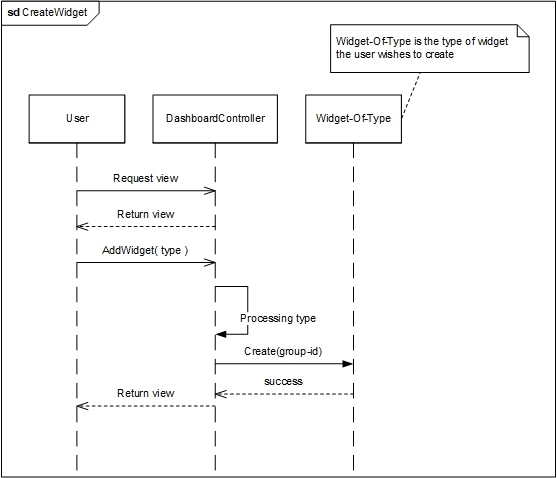
\includegraphics[width=1\textwidth]{09_Arkitektur/Dashboard/CreateWidgetSekvensjpg.jpg}
    \caption{Denne figur viser et sekvensdiagram der beskriver hvordan en vilkårlig widget oprettes. Herpå er widget-of-type lig med den type af widget der skal oprettes}
    \label{fig:CreateNewWidgetSeq}
\end{figure}

\jonathan{der er ikke mellemrum mellem anførselsteg og læses i nedenstående sætning}
Her skal "widget-of-type" læses, som den type af widget, man ønsker at oprette. Dashboardet kalder altså den controller der er tilknyttet den givne type af widget for at oprette en ny widget. Det kan på figuren ses, hvordan DashboardControlleren kommunikere med de andre controllere. Den fulde arkitektur for Dashboard kan findes i bilag \cite{ArkitekturDashboard}.

